\documentclass[10pt,pdf,hyperref={unicode}]{beamer}
\usepackage{amsmath, amsfonts}
\usepackage[utf8]{inputenc}
\usepackage[russian]{babel}
\usepackage{graphicx}
\usetheme{Warsaw}

\DeclareMathOperator{\svert}{\,\vert\,}
 
\setbeamertemplate{footline}[page number]{}
\setbeamertemplate{navigation symbols}{}

\hypersetup{pdfpagemode=FullScreen}
\author{Ефим Пышнограев}
\date{22 апреля 2014}
\institute{Филиал МГУ в городе Севастополе}
\title{Извлечение описаний событий предопределённых типов из потока сообщений пользователей микроблогов}

\begin{document}

\begin{frame}
  \titlepage
\end{frame}

\begin{frame}
  \frametitle{Введение}
  Цель работы:
  \begin{itemize}
	\item исследовать существующие подходы по извлечению описаний событий из сообщений пользователей, выделить возникающие проблемы и рассмотреть возможные методы их решения,
	\item исследовать возможность применения тематических моделей для решения задачи выявления событий,
	\item разработать метод для извлечения описаний событий из сообщений пользователей сети Твиттер на основе иерархического процесса Дирихле,
	\item протестировать работу алгоритма на реальных данных.
	\end{itemize}
\end{frame}

\begin{frame}
  \frametitle{Постановка задачи}
  Данные:
  \begin{itemize}
  	\item 
  	множество документов (сообщений) 
  	$\Omega = \left\{D_i \svert i \in \overline{1,n} \right\},$
	\item 
	документ --- множество слов и временная метка $t_i$ 
	$D_i = \left\{w_j \svert j \in \overline{ 1, l_i } \right\}.$
  \end{itemize}
  
  События:
  \begin{itemize}
	\item резкое увеличение частоты ключевых слов, затем спад до нормального уровня,
	\item должно быть вызвано реальным событием,
	\item не носит периодический характер.
  \end{itemize}
  
  Особенности сети Твиттер:
  \begin{itemize}
  \item короткие сообщения (до 140 символов),
  \item наличие шума и ошибок,
  \item большая плотность сообщений,
  \item ``взрывной'' характер событий.
  \end{itemize}
  
\end{frame}

\begin{frame}
  \frametitle{Схема алгоритма}
  Составные части:
  \begin{enumerate}  
  \item нахождение максимума в частотной функции, который будет соответствовать событию,
  \item извлечение ключевых слов, характерных этому максимуму,
  \item применение модели HDP с частичным обучением для того чтобы выделить все сообщения этой темы,
  \item проверка насколько полученный результат соответствует новому событию.
  \end{enumerate}
\end{frame}

\begin{frame}
  \frametitle{Результаты}
  Данные: 240 тысяч сообщений с 4 июня по 1 июля 2013 года, содержащие хэштег \#texas.
  \begin{figure}[H]
  \centering
  \includegraphics[width=5.0cm]{all-freq.eps}
  \includegraphics[width=5.0cm]{all-freq-scaled.eps}
  \end{figure}
\end{frame}

\begin{frame}
\frametitle{Результаты}
 Шаг 1: выделение экстремумов.
 \begin{figure}[H]
  \centering
  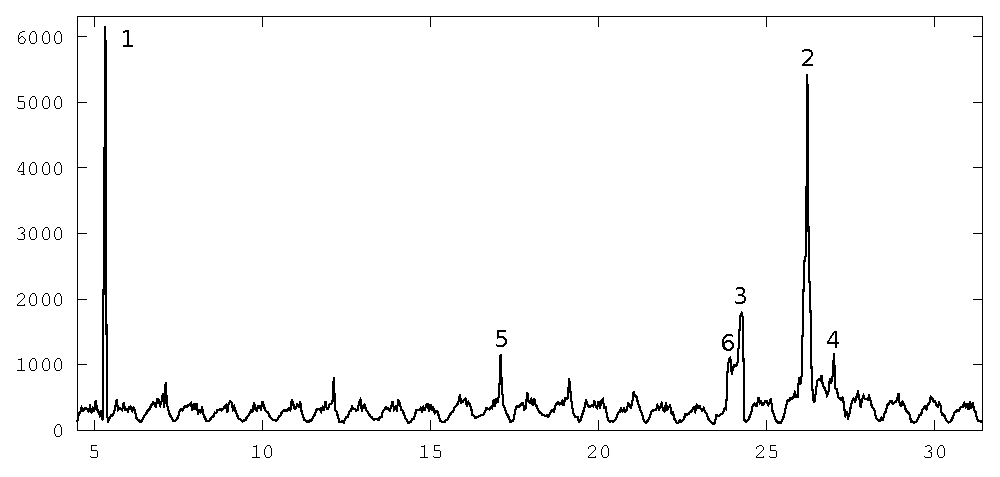
\includegraphics[width=10.0cm]{all-freq-labeled-1.eps}
  \label{fig:all-freq-labeled}
 \end{figure}
\end{frame}

\begin{frame}
\frametitle{Результаты}
Шаг 2: выделение ключевых слов.
\begin{table}
\begin{tabular}{r | l}
\#1 & year, read, prison, dragon, amazon, \\
\#2 & sb5, standwithwendi, talk, made, histori \\
\#3 & houston, california, england, artist, rt \\
\#4 & execut, 500th, mccarthi, kimberli, 1976 \\
\#5 & florida, z1, america, usa, bahrain \\
\#6 & houston, california, rt, watch, england \\
\end{tabular}
\end{table}	
\end{frame}

\begin{frame}
\frametitle{Результаты}
Шаг 3,\ 4: применение модели HDP, фильтрация.
\begin{figure}[H]
\centering
\includegraphics[width=5.0cm]{all-freq-5-8.eps}	
\includegraphics[width=5.0cm]{all-freq-26-5.eps}	

\includegraphics[width=5.0cm]{all-freq-24-6.eps}	
\includegraphics[width=5.0cm]{all-freq-27-0-1.eps}	

\includegraphics[width=5.0cm]{all-freq-17-2-1.eps}	
\includegraphics[width=5.0cm]{all-freq-23-20.eps}	
\end{figure}
\end{frame}

\begin{frame}
\frametitle{Результаты}
{\small
\begin{table}[H]
\centering		
\begin{tabular}{| l | l |}
	\hline
	 Ключевые слова & Вызвавшее событие \\ \hline
	 \begin{tabular}{l} year, read, prison, dragon, \\ amazon, written, bestseller \end{tabular} & \begin{tabular}{l} Написанная в техасской тюрьме книга \\ The Sword and the Dragon является \\ бестселлером на Amazon уже более трех \\ лет. \end{tabular} \\ \hline
	 \begin{tabular}{l} sb5, standwithwendi, abort, \\ senat \end{tabular} & \begin{tabular}{l} Обсуждение сенатом закона по запрету \\ абортов, который носит название Senate \\ Bill 5. Wendi Davis ---  политик, которая \\ боролась с принятием этого закона.  \end{tabular} \\ \hline
	 \begin{tabular}{l} houston, california, england, \\ artist, rt, watch, defjam \end{tabular} & \begin{tabular}{l} Хип хоп исполнитель из Хьюстон Devin \\ the Dude объявил, что его восьмой \\ студийный альбом будет называться \\ One for the Road и будет выпущен в \\ продажу в сентябре 2013 года. Альбом \\ будет выпущен лейблом Def Jam \\ Recordings.\end{tabular} \\ \hline
	 \begin{tabular}{l} execut, 500th, mccarthi, \\ kimberli, 1976\end{tabular} & \begin{tabular}{l} В штате Техас приведен в исполнение \\ 500-й по счету смертный приговор. \\ Смертная казнь имеет место с 1976 года.\end{tabular} \\ \hline
	\end{tabular}
\end{table}
}
\end{frame}

\begin{frame}
  \frametitle{Заключение}
  В ходе выполения дипломной работы было достигнуто:
	\begin{itemize}
	\item изучены существующие методы извлечения описаний событий из коротких пользовательских сообщений,
	\item изучена возможность применения тематических моделей для это задачи,
	\item разработан и проанализирован алгоритм извлечения описаний событий из социальной сети Твиттер на основе иерархического процесса Дирихле,
	\item алгоритм был реализован, параметры подобраны эксперементальным путем,
	\item тестирование показало, что алгоритм успешно распознает события, имеющиеся во входных данных.
	\end{itemize}
\end{frame}

\end{document}
